\onecolumn
\useRomanappendicesfalse
\appendices

\section{Proof of the Reward Guarantee}
\label{app:proof}

\begin{lemma}[Positive diagonal scaling]
\label{lem:diagonal}
Let $P\in\mathbb R_{\geq0}^{m\times n}$ and $\mathbf q\in\mathbb R_{>0}^{n}$.
With $t_i=(P^\top P\mathbf q)_i/q_i$, define the $i$-th column of $W$
as $P_{:i}/\sqrt{t_i}$ for $t_i>0$, and as zero otherwise.
Then $W\geq 0$ and $\|W\|_2\leq 1$.
\end{lemma}

\noindent\emph{Proof.}
Write $A=P^\top P$ and $T=\operatorname{diag}(\mathbf t)$.
The matrix $A$ is symmetric with nonnegative entries. For any
$\mathbf x\in\mathbb R^n$, expanding the square and using symmetry gives
\begin{align}
\mathbf x^\top(T-A)\mathbf x
&= \sum_i \frac{x_i^2}{q_i}\sum_j A_{ij}q_j
   - \sum_{i,j} A_{ij}x_i x_j \notag\\
&= \frac12\sum_{i,j}A_{ij}q_i q_j
       \left(\frac{x_i}{q_i}-\frac{x_j}{q_j}\right)^2
\ \geq\ 0.
\label{eq:diagonal_proof}
\end{align}
Thus $T\succeq P^\top P$, as in the diagonal construction of
Araujo et al.~\cite{araujo2023unified}. If $P_{:i}\neq 0$, then
$t_i\geq A_{ii}=\|P_{:i}\|_2^2>0$; if $P_{:i}=0$, then $t_i=0$.
On the nonzero columns, multiplying the matrix inequality on both sides by
$T^{-1/2}$ gives $W^\top W\preceq I$. Appending zero columns does not
change the operator norm. Nonnegativity follows from scaling each
nonzero column by a positive factor. \hfill$\square$

\medskip
\noindent\emph{Proof of Theorem~\ref{thm:reward}.}
Every linear layer is coordinatewise nondecreasing by Lemma~\ref{lem:diagonal}
and is $1$-Lipschitz in Euclidean norm; neither property depends on the bias.
Let $f(x)=\operatorname{ELU}(x)$ with unit shape parameter. MixedELU applies
one of $f(x)$, $-f(-x)$, or
\[
g(x)=
\begin{cases}
 f(x+1)-1, & x<0,\\
 1-f(1-x), & x\geq 0
\end{cases}
\]
to each channel. The branches are continuous, including at the joining
point $x=0$ in $g$, with slopes in $[0,1]$. Each scalar branch is therefore
nondecreasing and $1$-Lipschitz. Summing squared coordinate differences
gives the same Lipschitz bound for the coordinatewise activation in
Euclidean norm. Composition preserves both properties for $E_\theta$.

For $\mathbf z\leq\mathbf z'$ we have
$E_\theta(\mathbf z)\leq E_\theta(\mathbf z')$, so anchoring and
subtracting the energy in Eq.~\eqref{eq:mira_score} gives
$s_\theta(\mathbf z)\geq s_\theta(\mathbf z')$. The additive terms
$b+E_\theta(\mathbf 0)$ cancel from score differences, so the score
also has Lipschitz constant at most $1$. Finally, the derivative of
softplus is the sigmoid, which lies in $(0,1)$. Clipping the resulting
scalar at a fixed upper cap preserves monotonicity and cannot increase
any pairwise difference. Hence the reward is nonincreasing in each
error component and is $1$-Lipschitz. Since $\mathbf 0\leq\mathbf z$
for every valid input, $\mathbf 0$ maximizes the reward. \hfill$\square$

\medskip
\noindent\textbf{Scope.}
For fixed scales, Eq.~\eqref{eq:physical_normalization} also preserves
the componentwise ordering of the unnormalized error magnitudes.
In particular,
\[
\|\mathbf z^{(g)}\|_2
= \frac{\operatorname{RMS}(\mathbf e^{(g)})}{\max(\sigma_g,\epsilon)}.
\]
This identity explains the role of $\sqrt{d_g}$: repeating a group's
components does not increase the group's normalized norm when the scale
is fixed. The Euclidean bound is on $\mathbf z$, and the error scales
affect what it means for two inputs to be close. The theorem permits
ties, does not rank error vectors with opposing component changes,
and makes no guarantee about changes in policy actions or closed-loop
dynamics.

\clearpage
\section{Environment and Evaluation Protocol}
\label{app:protocol}

\begin{table}[!ht]
\caption{MIRA implementation settings for the evaluated humanoid.}
\label{tab:config}
\centering\small
\begin{tabular*}{0.91\linewidth}{@{\extracolsep{\fill}}ll@{}}
\toprule
Component & Setting \\
\midrule
Error and energy dimensions & $64\to341\to512\to1$; Box Carry uses $68$ input components \\
Discriminator & MixedELU, nonnegative diagonal-normalized linear weights \\
Error scale & Historical group means, floor $10^{-4}$, $\sqrt{d_g}$ scaling \\
Statistics collection & First $10^8$ environment samples \\
Policy and value networks & MLP with hidden widths $1024$ and $512$ \\
Policy and value optimizers & SGD, learning rate $10^{-4}$ \\
Discriminator optimizer & SGD, learning rate $2.5\times10^{-4}$, weight decay $10^{-4}$ \\
PPO & $\gamma=0.99$, GAE $0.95$, clipping $0.2$ at $30\,\mathrm{Hz}$ \\
Discriminator replay and regularization & $2\times10^5$ samples; output-weight regularizer $0.01$; no gradient penalty \\
\bottomrule
\end{tabular*}
\end{table}

\noindent\textbf{Reference and control.}
All configurations use the same humanoid model within a motion. The
actor observes current robot state and three future robot reference
frames. Sofa Sit uses the Sofa003 reference and a fixed sofa. Box Carry
uses a physics-recorded robot and box reference and a free $5$\,kg box.
The carry policy sees the box state and its position and linear velocity
targets three steps ahead. Its joint action is centered on the reference
joint target at the same preview time. The carry discriminator adds box
position and orientation errors and one hand-to-box position error per
hand. Soccer uses a run-up and shot adapted from CMU
motion~10\_02. A dynamic ball and a recorded PD command sequence are
shared across methods; the policies output residual targets around that
sequence. The evaluated Soccer configurations use $60\,\mathrm{Hz}$
control with four physics substeps per action, $\gamma=0.99^{1/2}$,
and GAE $0.95^{1/2}$.
The benchmark therefore measures reference tracking in these shared
control settings.

\medskip
\noindent\textbf{Windows and tracking errors.}
The three object-contact clips are evaluated from a fixed reference
start, using deterministic mean actions, with $256$ parallel simulator
replicas of each trained policy. The tracking errors average the
reference-aligned samples over time and replicas. For the logged
Backflip, Climb, and Roll results, we select tests whose reported mean
reference-start length reaches the respective horizon. Missing AMP
records remain unreported. Root and body position use Euclidean
distance, with body positions taken relative to the root. Root and body
orientation use geodesic rotation angles in world coordinates.
Velocity errors are mean absolute component differences. Reported body
errors average over all $15$ rigid bodies, whereas the reward's body
groups omit the separately represented root. Climb's matched
$299$-step records use $4.98$, $5.77$, and $7.86$ in units of $10^8$
environment samples for DeepMimic, ADD, and MIRA, respectively.
The other populated cells of Table~\ref{tab:per_motion_errors}
use $5.24\times10^8$ samples.

\medskip
\noindent\textbf{Motion-quality measures.}
Speed correlation is the mean across replicas of the Pearson
correlation between the reference and simulated planar root-speed
series. Speeds are planar displacements multiplied by the sample
rate after putting all traces on a $30\,\mathrm{Hz}$ grid.
Ground-support labels for each reference foot require the lowest sole
point to be at most $4$\,cm above the ground and the planar sole
center speed to be at most $0.15$\,m/s. Simulated support uses a
ground-normal contact force of at least $5$\,N. Let $S$ and $\hat S$
denote the respective sets of simulated and reference support
observations over feet, control steps, and replicas. Support timing
is $|S\cap\hat S|/|S\cup\hat S|$, and stance slip averages simulated
horizontal sole speed over $S\cap\hat S$. Scoring slip together with
IoU distinguishes low slip from simply avoiding contact.
Body jerk averages the Euclidean norm of the third finite difference
of world positions, divided by $(1/30\,\mathrm{s})^3$, over all body
points, replicas, and valid times on the $30\,\mathrm{Hz}$ grid.
It quantifies motion smoothness; it is independent of the reference
jerk. Each macro measure gives equal weight to the three motions.

\clearpage
\section{Per-Motion Results}
\label{app:motion_results}
The pose gains in the six-motion average in Table~\ref{tab:main} are
accompanied by mixed joint-velocity results. Roll has the largest
absolute joint-velocity gap to ADD, and Climb contributes the next
largest gap (Table~\ref{tab:per_motion_errors}). In the object-contact
subset, the two methods' mean joint-velocity errors are close:
$0.27922$\,rad/s for MIRA and $0.27845$\,rad/s for ADD.

% Generated by PAPER/tools/build_mira_supplement.py.
\begin{table}[!ht]
\caption{All seven tracking errors by motion. Each error is
lower-is-better; bold marks the minimum within a motion. A dash indicates
no full-window record.}
\label{tab:per_motion_errors}
\centering\small
\begin{tabular*}{\linewidth}{@{\extracolsep{\fill}}llrrrrrrr@{}}\toprule
Motion & Method & Root pos. & Root rot. & Body pos. & Body rot. & DoF vel. & Root vel. & Root ang. vel. \\
 &  & [m] & [rad] & [m] & [rad] & [rad/s] & [m/s] & [rad/s] \\
\midrule
Sofa Sit & AMP & 0.05643 & 0.05354 & 0.01898 & 0.08017 & 0.22264 & 0.04912 & 0.15148 \\
 & DeepMimic & 0.06289 & 0.06886 & 0.01939 & 0.10134 & 0.26330 & 0.06188 & 0.15906 \\
 & ADD & 0.04646 & 0.04788 & 0.02466 & 0.10496 & \textbf{0.20031} & 0.05911 & 0.12598 \\
 & MIRA & \textbf{0.02510} & \textbf{0.03493} & \textbf{0.01756} & \textbf{0.07354} & 0.21265 & \textbf{0.04435} & \textbf{0.09390} \\
\midrule
Box Carry & AMP & 0.06527 & 0.07425 & 0.02919 & 0.11726 & 0.34581 & 0.08315 & 0.24272 \\
 & DeepMimic & 0.03610 & 0.07578 & 0.02603 & 0.12043 & 0.39081 & 0.07569 & 0.23779 \\
 & ADD & 0.03294 & \textbf{0.02914} & \textbf{0.01409} & \textbf{0.05079} & \textbf{0.24308} & 0.05340 & 0.14942 \\
 & MIRA & \textbf{0.01758} & 0.03004 & 0.01454 & 0.06598 & 0.26419 & \textbf{0.04009} & \textbf{0.12313} \\
\midrule
Soccer & AMP & 0.19943 & 0.18676 & 0.04121 & 0.17498 & 0.48696 & 0.16281 & 0.45426 \\
 & DeepMimic & 0.05825 & 0.12887 & 0.03811 & 0.14462 & 0.52029 & 0.14136 & 0.48188 \\
 & ADD & 0.09080 & 0.15837 & 0.05410 & 0.16350 & 0.39195 & 0.18259 & 0.42422 \\
 & MIRA & \textbf{0.04255} & \textbf{0.07100} & \textbf{0.02209} & \textbf{0.08950} & \textbf{0.36081} & \textbf{0.06791} & \textbf{0.23764} \\
\midrule
Backflip & AMP & \textemdash & \textemdash & \textemdash & \textemdash & \textemdash & \textemdash & \textemdash \\
 & DeepMimic & \textbf{0.05372} & 0.09874 & 0.03963 & 0.17924 & 1.29761 & \textbf{0.26989} & 0.76622 \\
 & ADD & 0.09050 & 0.08918 & 0.04373 & \textbf{0.16523} & 1.04228 & 0.35286 & 0.60606 \\
 & MIRA & 0.05440 & \textbf{0.03033} & \textbf{0.03734} & 0.17010 & \textbf{0.97935} & 0.27595 & \textbf{0.23157} \\
\midrule
Climb & AMP & \textemdash & \textemdash & \textemdash & \textemdash & \textemdash & \textemdash & \textemdash \\
 & DeepMimic & 0.08136 & 0.12284 & 0.05133 & 0.21424 & 0.77060 & 0.17078 & 0.45419 \\
 & ADD & 0.07485 & 0.04093 & \textbf{0.02309} & \textbf{0.08719} & \textbf{0.49826} & 0.11936 & 0.29386 \\
 & MIRA & \textbf{0.05190} & \textbf{0.03655} & 0.02499 & 0.09556 & 0.54729 & \textbf{0.09801} & \textbf{0.23404} \\
\midrule
Roll & AMP & 0.56447 & 1.66980 & 0.44628 & 1.53132 & 2.34323 & 0.73310 & 2.14431 \\
 & DeepMimic & 0.17524 & 0.40429 & 0.14525 & 0.51261 & 1.31412 & 0.34178 & 0.73293 \\
 & ADD & 0.07787 & 0.09266 & \textbf{0.03989} & \textbf{0.13888} & \textbf{0.83377} & 0.32784 & 0.55320 \\
 & MIRA & \textbf{0.07446} & \textbf{0.06211} & 0.04671 & 0.17127 & 0.95091 & \textbf{0.30073} & \textbf{0.45582} \\
\bottomrule\end{tabular*}
\end{table}


% Generated by PAPER/tools/build_mira_supplement.py.
\begin{table}[!ht]
\caption{Motion quality by motion. Ground support is
foot--ground contact, including in the sofa and box scenes.}
\label{tab:per_motion_quality}
\centering\small
\begin{tabular*}{\linewidth}{@{\extracolsep{\fill}}llrrrr@{}}\toprule
Motion & Method & Speed $r$ $\uparrow$ & Support IoU [\%] $\uparrow$ & Stance slip [cm/s] $\downarrow$ & Jerk [m/s$^3$] $\downarrow$ \\
\midrule
Sofa Sit & AMP & 0.9745 & 60.15 & 1.006 & 59.88 \\
 & DeepMimic & 0.9837 & 59.54 & 1.538 & 65.71 \\
 & ADD & 0.9811 & 48.59 & \textbf{0.882} & 64.52 \\
 & MIRA & \textbf{0.9870} & \textbf{61.60} & 1.515 & \textbf{57.69} \\
\midrule
Box Carry & AMP & 0.9651 & 75.05 & 2.639 & 124.60 \\
 & DeepMimic & 0.9665 & 75.04 & 0.963 & \textbf{110.31} \\
 & ADD & 0.9822 & \textbf{77.84} & 1.759 & 124.16 \\
 & MIRA & \textbf{0.9926} & 76.12 & \textbf{0.920} & 128.05 \\
\midrule
Soccer & AMP & 0.9755 & 83.47 & 4.977 & 337.46 \\
 & DeepMimic & 0.9729 & 74.33 & 3.490 & 348.45 \\
 & ADD & 0.8318 & 75.68 & 3.820 & 336.60 \\
 & MIRA & \textbf{0.9946} & \textbf{86.20} & \textbf{2.720} & \textbf{327.76} \\
\bottomrule\end{tabular*}
\end{table}


\noindent In the contact subset, MIRA obtains the strongest speed
correlation for each motion. The lower mean stance slip is driven by
Box Carry and Soccer; ADD has lower stance slip on Sofa Sit. For Box
Carry, ADD has the highest support IoU, and DeepMimic has the lowest
jerk. These per-motion comparisons distinguish the macro gains from
performance on any individual clip.

\clearpage
\section{Learning Dynamics}
\label{app:dynamics}
The curves below use training-time reference-start tests. Their horizontal
axis counts actual environment samples rather than progress relative to
each run's final iteration. Figure~\ref{fig:learning} averages the six
motions equally up to their shared base sample budget. Values between
logged tests are linearly interpolated using the same sample grid.
Tracking errors in these logs are computed on executed timesteps. For
that reason, a low early error can describe a partially tracked
reference; the curves alone cannot establish full-motion fidelity.
The aligned endpoints in Table~\ref{tab:per_motion_errors} answer that
separate question.

\begin{figure}[!ht]
\centering
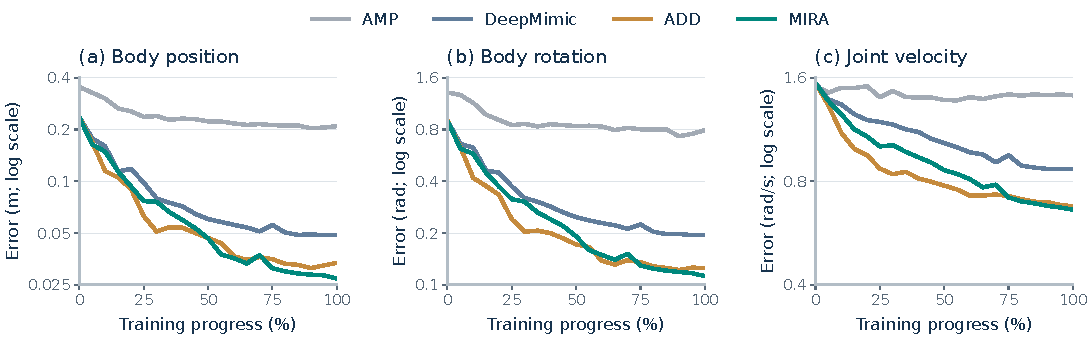
\includegraphics[width=\linewidth]{figures/mira_tracking_curves.pdf}
\caption{Body-position, body-rotation, and joint-velocity errors averaged
over the six motions at equal training sample counts. Lower is better.}
\label{fig:learning}
\end{figure}

\noindent Figure~\ref{fig:velocity_detail} examines joint-velocity
errors for Roll and Climb, where MIRA's largest terminal differences
to ADD occur. The longer Climb runs continue to their last recorded
tests; no continuation is inferred for runs that stop earlier.
A portion of the Climb curves, particularly early in training,
describes trajectories shorter than $299$ steps.

\begin{figure}[!ht]
\centering
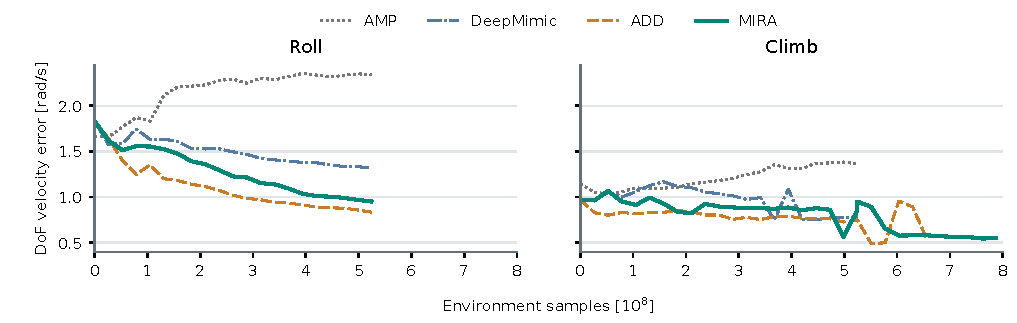
\includegraphics[width=\linewidth]{figures/mira_roll_climb_velocity.pdf}
\caption{Joint-velocity error during training on Roll and Climb.
The ADD Climb curve includes its continuation.}
\label{fig:velocity_detail}
\end{figure}

\clearpage
\section{Complete Backflip Ablations}
\label{app:ablation}
We evaluate all six checkpoints on Backflip from the reference start
with deterministic mean actions and no automatic resets. Each trained
for $5.24\times10^8$ samples. The compared windows are steps 1--60
for variants with a full trace, and steps 1--26 for all variants.
The two variants without diagonal normalization end at $26$ and
$28$ steps. Neither contributes a full-window error. Each checkpoint
is evaluated in $256$ simulator replicas.

% Generated by PAPER/tools/build_mira_supplement.py.
\begin{table}[!ht]
\caption{All tracking errors for Backflip ablations. Each panel
uses one prefix common to every row in that panel. Units match
Table~\ref{tab:per_motion_errors}; lower is better.}
\label{tab:full_ablation}
\centering\small
\setlength{\tabcolsep}{3pt}
\begin{tabular*}{\linewidth}{@{\extracolsep{\fill}}lrrrrrrr@{}}\toprule
Configuration & Root pos. & Root rot. & Body pos. & Body rot. & DoF vel. & Root vel. & Root ang. vel. \\
\midrule
\multicolumn{8}{@{}l}{\textit{Steps 1--60}} \\
MIRA & \textbf{0.0560} & \textbf{0.0314} & \textbf{0.0386} & \textbf{0.1758} & \textbf{1.0112} & \textbf{0.2849} & \textbf{0.2378} \\
Signed weights & 0.0593 & 0.0406 & 0.0418 & 0.1841 & 1.0828 & 0.3020 & 0.2695 \\
No $\sqrt{d_g}$ scaling & 0.0758 & 0.1885 & 0.0788 & 0.2888 & 1.2346 & 0.4780 & 0.7948 \\
Signed input & 0.1267 & 0.1312 & 0.0716 & 0.3162 & 1.8406 & 0.3854 & 0.9466 \\
\midrule
\multicolumn{8}{@{}l}{\textit{Steps 1--26}} \\
MIRA & 0.0660 & \textbf{0.0275} & \textbf{0.0442} & \textbf{0.2117} & \textbf{1.0913} & 0.2706 & \textbf{0.2412} \\
Signed weights & 0.0694 & 0.0377 & 0.0484 & 0.2222 & 1.1809 & 0.3082 & 0.2790 \\
No $\sqrt{d_g}$ scaling & \textbf{0.0583} & 0.1115 & 0.0632 & 0.2718 & 1.2323 & 0.3568 & 0.7199 \\
No diagonal normalization & 0.0680 & 0.1150 & 0.0664 & 0.2722 & 1.5976 & 0.2949 & 0.8751 \\
Signed input & 0.0849 & 0.1264 & 0.0759 & 0.3467 & 2.1448 & 0.3507 & 0.9597 \\
Signed input + no diagonal norm. & 0.0678 & 0.0775 & 0.0524 & 0.2156 & 1.4135 & \textbf{0.2687} & 0.6668 \\
\bottomrule\end{tabular*}
\end{table}


\noindent\textbf{Controls and combined perturbations.}
The signed-weight variant retains physical errors, group scaling,
and the effective nonnegative initialization. Its diagonal scaling is
applied to magnitudes, so its signed effective matrix $W_s$ satisfies
$\|W_s\mathbf x\|_2\leq\||W_s|\,|\mathbf x|\|_2\leq\|\mathbf x\|_2$.
The \emph{Signed input} variant changes the representation to the
$172$-component signed differential with per-coordinate scale estimates
and permits signed weights. It uses signed-compatible diagonal
normalization, and therefore measures a joint representation and
network change. We additionally combine it with removing diagonal
normalization. The same output-weight penalty coefficient applies in
all variants, but the unnormalized output head can change its norm.

\begin{figure}[!ht]
\centering
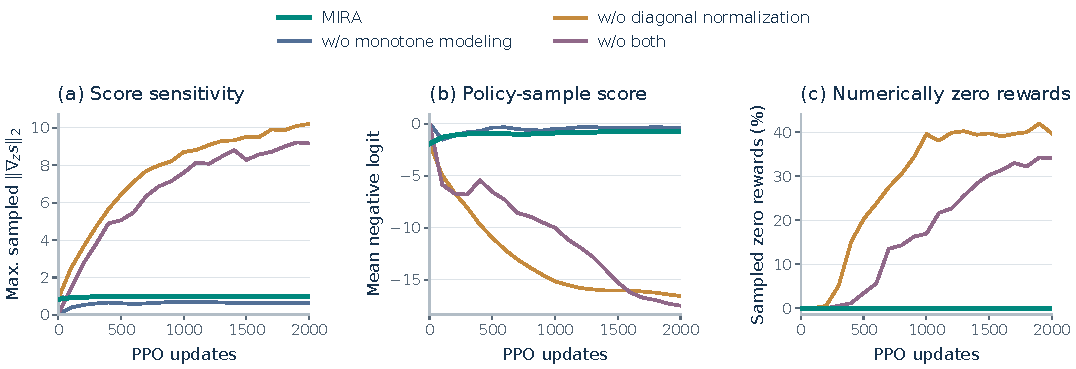
\includegraphics[width=\linewidth]{figures/mira_discriminator_diagnostics.pdf}
\caption{Backflip discriminator diagnostics from the seed-0 training runs.
Each model is probed on its own rollouts. Input-gradient norms are in the
model's normalized input coordinates.}
\label{fig:diagnostics}
\end{figure}

\noindent\textbf{Critic behavior.}
For the two variants sharing the physical error representation,
the terminal maximum sampled score-gradient norm is $0.995$ for
MIRA and $10.214$ without diagonal normalization, and numerically
zero rewards increase from $0\%$ to $39.72\%$ of samples.
These are local measurements on different rollouts; they connect the
constraint to the critic's score and reward ranges. Norms for the
signed-differential input refer to different coordinates. Neither
the diagnostic curves nor the rollout replicas quantify variation
across independent training seeds.
